%!TEX root =  cl2-lda.tex

Predicting users' reactions to the debate based on n-grams from the text of the each turn taken by the candidates is a simple approach, and we are interested to see how well the topic-based methods compare to it in terms of performance.

On all the tasks, we predict the responses to turns using Decision Tree, Maximum Entropy and Naive Bayes classifiers; we used the implementations of these classifiers from NLTK~\cite{bird_nltk:_2006}.  We measure our final accuracy on all tasks with 10-fold cross validation.  

To extract n-gram features from the transcripts of the turns, we begin by splitting the text into tokens using the English tokenizer from NLTK.  We then remove punctuation, numbers and stop-words; and then convert all n-grams to lower-case.  Finally, we produce a single feature for each unique n-gram in each turn indicating its presence (not the count of tokens for that n-gram).  

For our evaluation, we consider either unigrams or bigrams as features.  To determine the number of n-gram features to use to avoid overfitting, we vary their number while evaluating mean accuracy during repeated random sub-sampling validation.  To select which n-grams to include among the features, we select the most frequent n-grams first.  We also remove very short turns (less than thirty words long) from the set of examples for training and testing.

\begin{table}[]
\begin{centering}
\begin{tabular}{ l | l | l }
Classifier & Obama voters & Romney voters \\
\hline
DecTree & \textbf{0.65} (0.14) &  \textbf{0.58} (0.17) \\
MaxEnt & \textbf{0.57} (.14) &  \textbf{.68} (.16) \\
Naive & \textbf{0.57} (.17) &  \textbf{.67} (.15) \\
\end{tabular}
\caption{Task 1 (unigram features): Accuracy and StdDev}
\label{tab:task1unigrams}
\end{centering}
\end{table}

\begin{figure}[]
	\centering
	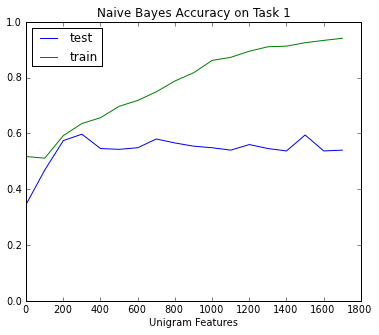
\includegraphics[scale=0.55]{Figures/ngrams_hyperparam_task1.png}
	\caption{Unigrams hyperparameter tuning for Task 1 Naive Bayes for Obama supporter reactions.}
	\label{fig:ngramstask1hyperparam}
\end{figure}

First we consider results with unigram features. In Table~\ref{tab:task1unigrams} we see that on \textbf{Task 1} we see that all three classifiers performed similarly.  This task is challenging for the classifiers, for example with the Naive Bayes model we see in Fig.~\ref{fig:ngramstask1hyperparam} that test accuracy quickly reaches a limit as we consider much more than a few hundred unigram features and the model quickly overfits due to the relatively high number of features per training example.

In contrast, the models are substantially more successful on \textbf{Task 2}.  Interestingly the Naive Bayes model performed very well when predicting reactions of Obama voters, cf.~\ref{fig:ngramstask2hyperparam} -- the most informative features where \emph{Romney} and \emph{Governor}, perhaps because the words are more often said by their chosen candidate than the opponent.  But, it did not perform well for Romney voters, cf. Table~\ref{tab:task2unigrams} -- here the most informative feature was \emph{idea}, which doesn't seem to have as much clear meaning as the name of an opponent. 

\begin{figure}[]
	\centering
	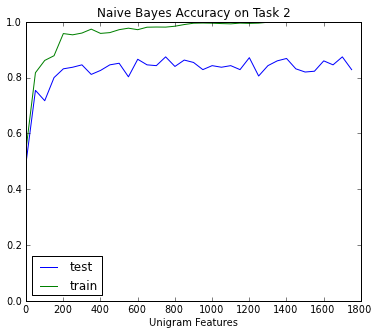
\includegraphics[scale=0.60]{Figures/ngrams_hyperparam_task2.png}
	\caption{Unigrams hyperparameter tuning for Task 1 Naive Bayes for Obama supporter reactions.}
	\label{fig:ngramstask2hyperparam}
\end{figure}

\begin{table}[]
\begin{centering}
\begin{tabular}{ l | l | l }
Classifier & Obama voters & Romney voters \\
\hline
DecTree & \textbf{0.74} (0.22) &  \textbf{0.83} (0.12) \\
MaxEnt & \textbf{0.76} (.16) &  \textbf{.80} (.06) \\
Naive & \textbf{0.87} (.12) &  \textbf{.50} (.12) \\
\end{tabular}
\caption{Task 2 (unigram features): Accuracy and StdDev}
\label{tab:task2unigrams}
\end{centering}
\end{table}

Something that may help to explain this difference is an interesting difference between the over-all reactions of the Obama supporters and Romney supporters over all turns.  In Fig.~\ref{fig:ngramsbalanceoba} we see frequency distribution of ratios of reactions in agreeing with Obama to the reactions disagreeing.  There are four clear modes in this distribution.  From left-to-right on the x-axis, the first mode reflects turns in which Obama supporters strongly \emph{disagreed} with what was being said, the next two modes reflect turns in which they slightly disagreed or slightly \emph{agreed}, respectively, and the right-most mode represents turns when Obama supporters agreed very strongly.

\begin{figure}[]
	\centering
	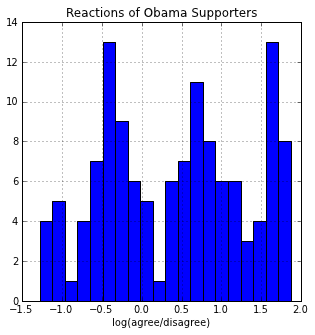
\includegraphics[scale=0.60]{Figures/ngrams_balance_oba.png}
	\caption{The ratio of agreeing reactions to disagreeing reactions among Obama supporters throughout the debate.}
	\label{fig:ngramsbalanceoba}
\end{figure}

Now contrast this with the corresponding distribution of Romney supporter reactions in Fig.~\ref{fig:ngramsbalancerom}.  The patterns that emerges is that the mode in distribution representing strong disagreement is gone from the Republican supporters and the mode representing strong support is higher (in relative but not absolute numbers, because the number of Obama supporters outnumber the Romney supporters).  As a consequence, there is a greater bias in the training sets for the Naive Bayes classifier on Task 2, which -- in combination with a small training size over-all -- can lead to a tendency to predict the common class regardless of the features.  Another reason for the difference in performance may be the difference in numbers of Obama supporters and Romney supporters in the data set, such that there is a clearer signal of consensus over topics (here, unigrams) that Obama supporters react to, and a tendency to over-fit.  Indeed, we see in Fig.~\ref{fig:ngramstask2hyperparamrom} that the Naive Bayes model over fits easily as we increase the number of unigram features.

\begin{figure}[]
	\centering
	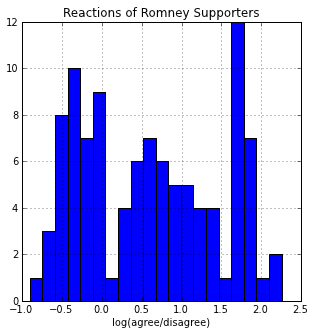
\includegraphics[scale=0.60]{Figures/ngrams_balance_rom.png}
	\caption{The ratio of agreeing reactions to disagreeing reactions among Romney supporters throughout the debate.}
	\label{fig:ngramsbalancerom}
\end{figure}

\begin{figure}[]
	\centering
	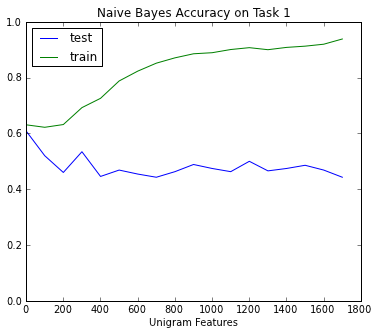
\includegraphics[scale=0.60]{Figures/ngrams_hyperparam_task2_rom.png}
	\caption{Unigrams hyperparameter tuning for Task 1 Naive Bayes for Romney supporter reactions.}
	\label{fig:ngramstask2hyperparamrom}
\end{figure}

Continuing, we see in~\ref{tab:task3unigrams} that on \textbf{Task 3}, Maximum Entropy performed best over all while Naive Bayes continued to struggle at predicting reactions of Romney voters.

\begin{table}[]
\begin{centering}
\begin{tabular}{ l | l | l }
Classifier & Obama voters & Romney voters \\
\hline
DecTree & \textbf{0.83} (0.14) &  \textbf{0.80} (0.15) \\
MaxEnt & \textbf{0.86} (.09) &  \textbf{.84} (.13) \\
Naive & \textbf{0.81} (.11) &  \textbf{.49} (.23) \\
\end{tabular}
\caption{Task 3 (unigram features): Accuracy and StdDev}
\label{tab:task3unigrams}
\end{centering}
\end{table}

Bigram features consistently underperform the unigram features, which is not surprising since there were very training examples over all, permitting over-fitting if we increase the number of bigram features, and the models are not smoothed which is aggravated by the use of bigram features rather than unigram features.  Table~\ref{tab:task1bigrams} reveals poor performance on \textbf{Task 1} for Obama supporters by all classifiers; interestingly, Romney supporters' reactions were more easily predicted in this setting.  The most informative bigram feature to predict strong reactions from Romney supporters on \textbf{Task 1} was \emph{cut taxes}, which is easily understood as a meaningful collocation in general and for this group in particular. The most informative bigram to predict low reactions is \emph{Governor Romney}, perhaps because this is most often said by the moderator or the other candidate rather than Romney himself.  \textbf{Task 2} and \textbf{Task 3} continued to perform poorly over all with bigram features, cf. Table~\ref{tab:task2bigrams} and Table~\ref{tab:task3bigrams}.

\begin{table}[H]
\begin{centering}
\begin{tabular}{ l | l | l }
Classifier & Obama voters & Romney voters \\
\hline
DecTree & \textbf{0.40} (0.12) &  \textbf{0.73} (0.12) \\
MaxEnt & \textbf{0.60} (.14) &  \textbf{.73} (.10) \\
Naive & \textbf{0.60} (.11) &  \textbf{.73} (.17) \\
\end{tabular}
\caption{Task 1 (bigram features): Accuracy and StdDev}
\label{tab:task1bigrams}
\end{centering}
\end{table}

\begin{table}[H]
\begin{centering}
\begin{tabular}{ l | l | l }
Classifier & Obama voters & Romney voters \\
\hline
DecTree & \textbf{0.46} (0.18) &  \textbf{0.63} (0.13) \\
MaxEnt & \textbf{0.54} (.11) &  \textbf{.63} (.17) \\
Naive & \textbf{0.44} (.22) &  \textbf{.63} (.21) \\
\end{tabular}
\caption{Task 2 (bigram features): Accuracy and StdDev}
\label{tab:task2bigrams}
\end{centering}
\end{table}

\begin{table}[H]
\begin{centering}
\begin{tabular}{ l | l | l }
Classifier & Obama voters & Romney voters \\
\hline
DecTree & \textbf{0.50} (0.09) &  \textbf{0.60} (0.19) \\
MaxEnt & \textbf{0.50} (.24) &  \textbf{.40} (.22) \\
Naive & \textbf{0.33} (.13) &  \textbf{.60} (.11) \\
\end{tabular}
\caption{Task 3 (bigram features): Accuracy and StdDev}
\label{tab:task3bigrams}
\end{centering}
\end{table}